%\newpage
\section{Tieftöner-Messungen} \label{sec:5.3}
\subsection{Einleitung} \label{subsec:5.3.1}
Tieftöner sind, wie der Name bereits andeutet, für den unteren Frequenzbereich gedacht und konzipiert.
In diesem Projekt werden Tieftöner-Lautsprecher an zwei verschiedenen Positionen verwendet:
\begin{itemize}
	\item Im Subwoofer und 
	\item in der Satellitenbox
\end{itemize}
Es ist so angedacht, dass der Subwoofer (Mono) nur die sehr niedrigen Frequenzen übernimmt.
Er ist bis ca. 200 Hz aktiv.\\
In den Satellitenboxen ist jeweils ein kleinerer Tieftöner verbaut, um den Übergang zwischen sehr tiefen und hohen Frequenzen zu bilden.
Diese zwei Lautsprecher (Stereo) arbeiten ebenfalls bei niedrigen als auch bei mittleren bis hohen Frequenzen.
Die Grenze des Satelliten-Tieftöners liegt bei ca. 5 kHz.

\subsection{Ziele} \label{subsec:5.3.2}
Der Lautsprecher für die Subwoofer-Box muss größer und leistungsfähiger sein, um die richtig tiefen Frequenzen möglichst gut abzustrahlen.
Da er nur bis ca. 200 Hz aktiv ist, sollte der Frequenzgang genau in diesem Bereich einen hohen Schalldruckpegel aufweisen.
Der Rest des Frequenzganges ist nicht so wichtig, da der Lautsprecher auch nicht in einem höheren Bereich verwendet wird. \\
Bei den Satelliten-Lautsprechern ist der ganz tiefe Frequenzbereich nicht so ausschlaggebend.
Wichtiger ist dafür eine niedrige Welligkeit bis 5 kHz, um den mittleren Frequenzbereich gut abstrahlen zu können.\\ \\
%Welligkeit könnte man vielleicht auch erklären als Grundlage -- @Bointii
Der Messvorgang und -aufbau wurde bereits im Kapitel \ref{sec:5.2} erläutert.
Nach diesem Prinzip wird bei fast allen Messungen vorgegangen.

\newpage
\subsection{Subwoofer} \label{subsec:5.3.3}
Bereits zu Beginn der Diplomarbeit wurde ein großer Tieftöner eingekauft.\\
Dieser wurde in verschiedenen Volumina gemessen.\\
Außerdem wurden Vergleichsmessungen mit einem zweiten Tieftöner durchgeführt.
\begin{figure} [H]
	\centering
	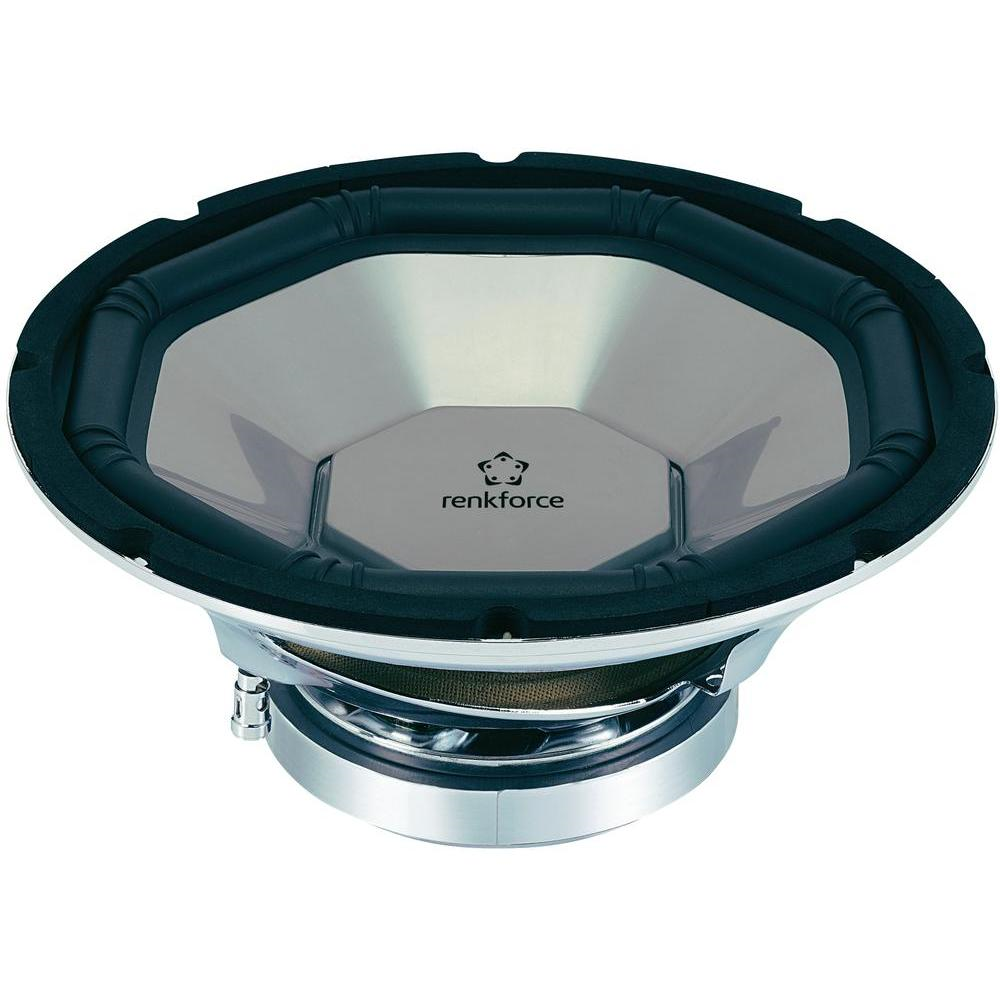
\includegraphics[width=0.5\textwidth]{img/LSMessung/TT/renkforce_B12123.png}
	\caption[\enquote{Renkforce B12123}]{\enquote{Renkforce B12123}\footnotemark}
	\label{fig:5.3.3.1}
\end{figure}
\footnotetext{https://www.conrad.at/de/auto-subwoofer-chassis-300-mm-500-w-renkforce-4-370335.html}
Dieser Lautsprecher wurde ausgewählt, weil er einen vergleichsweise hohen Schalldruckpegel bei tiefen Frequenzen aufweist.
Kurze Spezifikationen des Subwoofers sind:
\begin{itemize}
	\item Maximale Belastbarkeit 500 W
	\item Durchmesser 30 cm
	\item Schalldruck 93 dB
	\item Impedanz 4 $\Omega$
\end{itemize}
Da man eine Box einfacher verkleinern kann als vergrößern, wurde eine Box mit einem Volumen von 149 l für die Messungen verwendet.
Die Box wurde aus Holz gefertigt und mit Silikon abgeschlossen, um mögliche Luftlöcher zu schließen.
Als Vergleichslautsprecher wurde ein \enquote{Visaton WPC30} gemessen.

\newpage
Diese Messungen wurden zu Beginn der Diplomarbeit durchgeführt und daher sind die Ergebnisse so aufgenommen, dass die Einstellungen der Software sichtbar sind.\\ % Ideale Messung beschreiben?
Die zwei Subwoofer wurden einmal mit und einmal ohne Wolle in der Box gemessen. 
\begin{figure} [H]
	\centering
	\subfloat{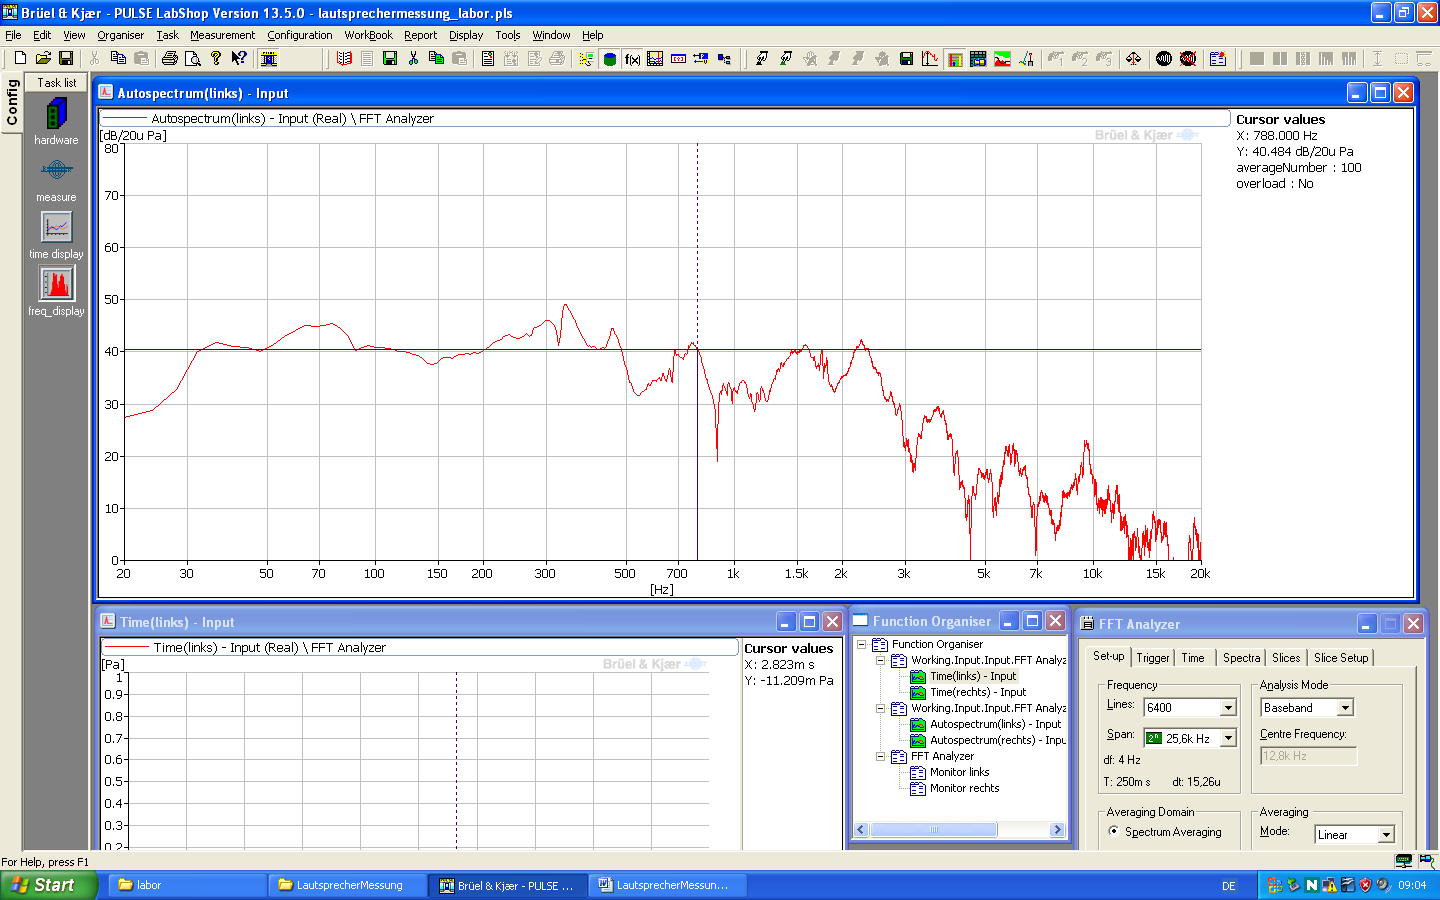
\includegraphics[width=0.75\textwidth]{img/LSMessung/TT/RenkforceOhneWolleMitSilikon.png}}\quad
	\subfloat{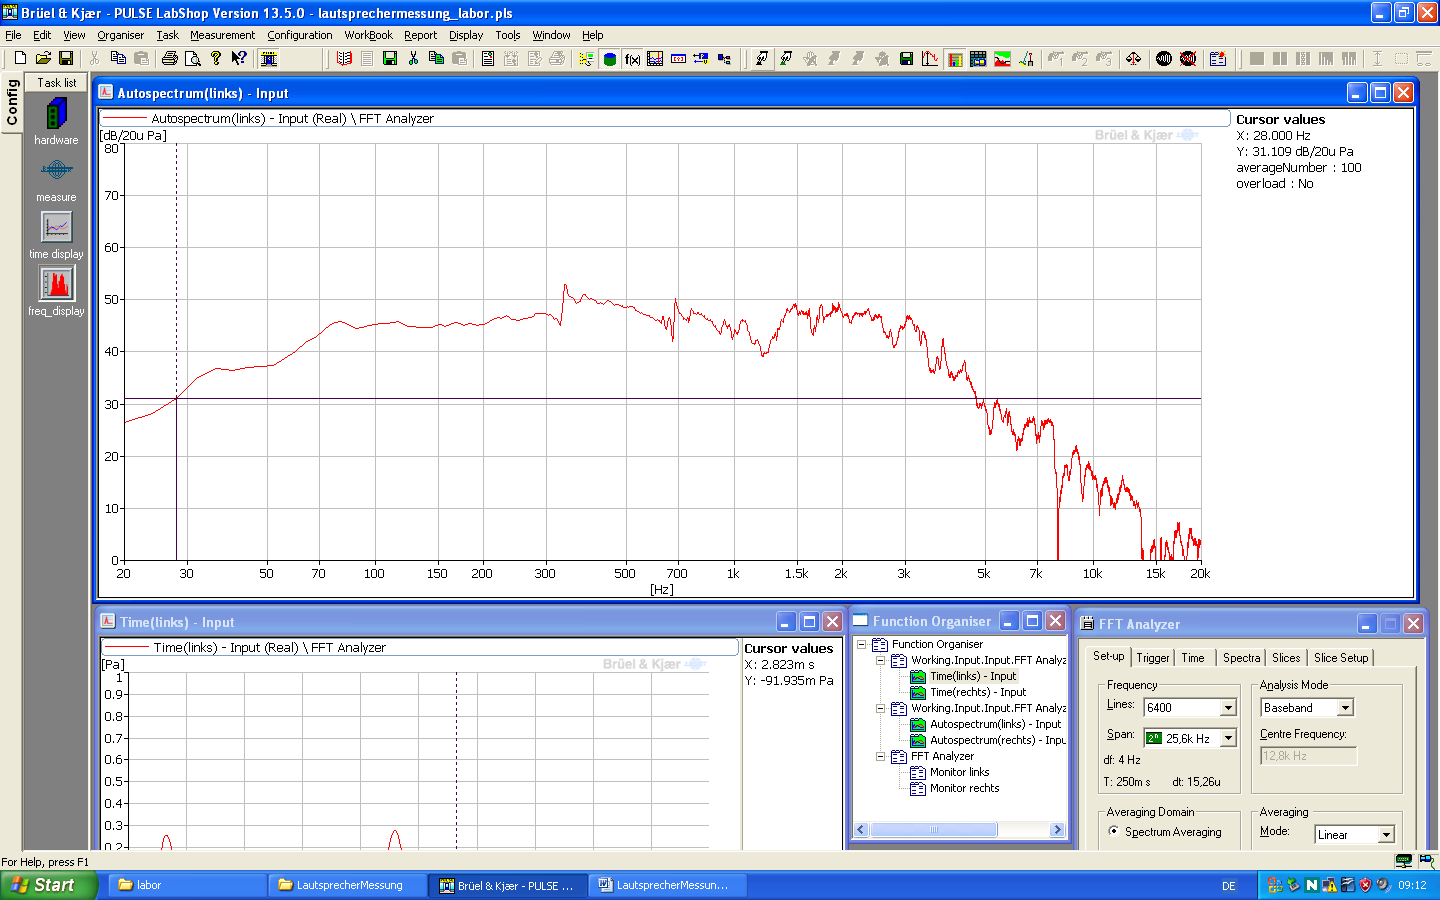
\includegraphics[width=0.75\textwidth]{img/LSMessung/TT/VisatonMitSilikonOhneWolle.png}}
	\caption{Subwoofer-Messung ohne Wolle\\ \enquote{Renkforce} (oben) und \enquote{Visaton} (unten)}
	\label{fig:5.3.3.2}
\end{figure}
Bei diesem Vergleich ist sichtbar, dass der Frequenzgang des \enquote{Visaton}-Tieftöners allgemein \enquote{gerader} ist und weniger Welligkeit aufweist.
Wenn man allerdings nur auf die tiefen Frequenzen achtet, die auch verwendet werden (<200 Hz), ist festzustellen, dass der Schalldruckpegel des \enquote{Renkforce} einen höheren Wert aufweist und daher zu bevorzugen ist.\\
Eine weitere Messung mit Wolle in der Box wurde deshalb durchgeführt, weil beide Frequenzgänge bei ca. 300 Hz einen Unregelmäßigkeit aufzeigen.
Die Auswirkungen auf die Lautsprecher sind folgende:
\begin{figure} [H]
	\centering
	\subfloat{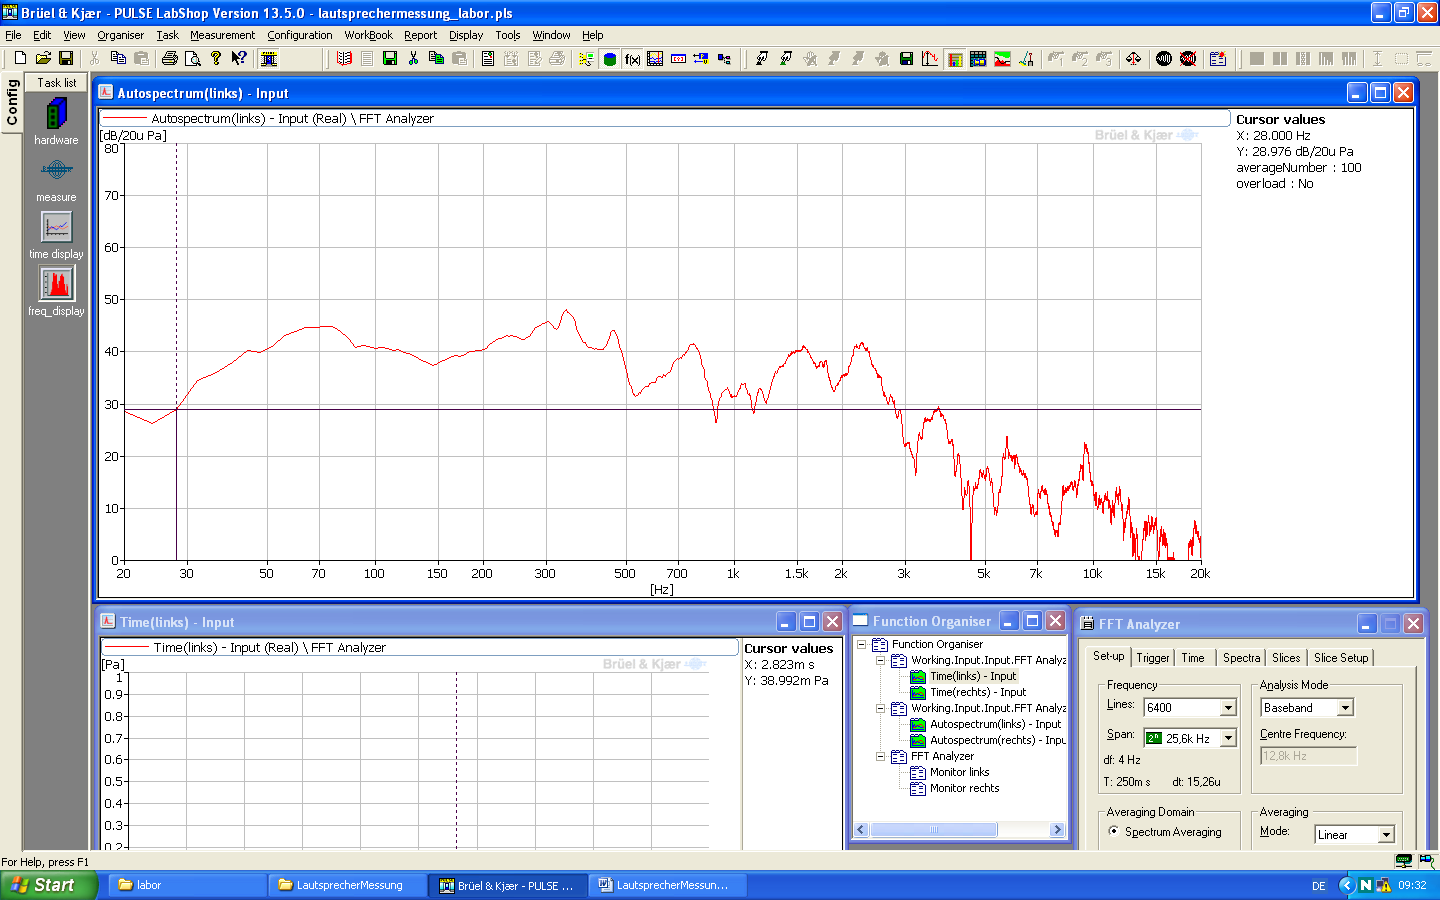
\includegraphics[width=0.75\textwidth]{img/LSMessung/TT/RenkforceMitWolleMitSilikon.png}}\quad
	\subfloat{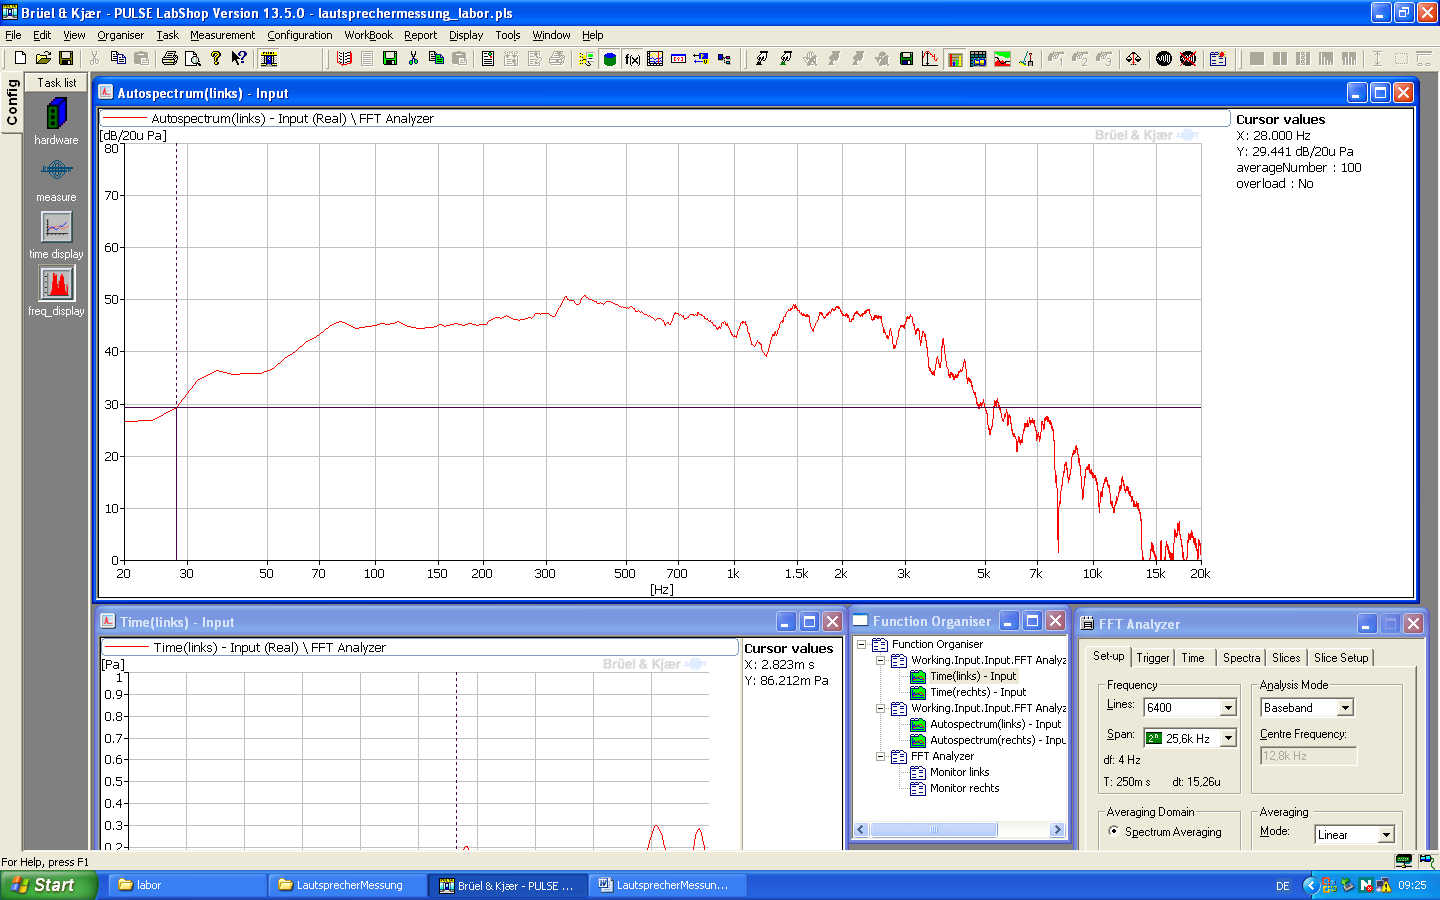
\includegraphics[width=0.75\textwidth]{img/LSMessung/TT/VisatonMitSilikonMitWolle.png}}
	\caption{Subwoofer-Messung mit Wolle\\ \enquote{Renkforce} (oben) und \enquote{Visaton} (unten)}
	\label{fig:5.3.3.3}
\end{figure}
Beide Frequenzgänge wurden durch das Hinzufügen von Wolle etwas \enquote{glatter}, also haben weniger Welligkeit.
Die Wolle kann z.B. stehende Wellen in der Box verhindern und verbessert so deshalb die Eigenschaften der gesamten Box.\\ \\	%Es wirkt wie eine Vergrößerung des Volumens - hat Wagn einmal gsagt
Der Lautsprecher \enquote{Renkforce} weist insgesamt bei tieferen Frequenzen einen höheren Schalldruckpegel auf und wurde auch deshalb von uns für dieses Projekt ausgewählt.


\subsection{Satelliten-Tieftöner} \label{5.3.4}
Als Satelliten-Tieftöner kommen mehrere Lautsprecher in frage, diese vom Betreuer zu Verfügung gestellt wurden.
Die Lautsprecher-Chassis haben einen ähnlichen Durchmesser.
Dadurch können sie in einem Gehäuse (à 13,72 Liter) mit wechselbarer Frontplatte gemessen werden.
Um möglicherweise bessere Ergebnisse erzielen zu können wurde das Volumen mittels (Ziegel, Styropor, Ytong) verringert oder durch Wolle vergrößert.\\
Zu den gemessenen Chassis gehören:
\begin{itemize}
	\item \enquote{TT1}: PSS 297 58206 100W 6Ohm
	\item \enquote{TT2}: SAMCO 10D1K06 20W 8Ohm
%	\item \enquote{TT3}: Infinity, ein Auto-Lautsprecher
\end{itemize}
Die Bezeichnung TT1 und TT2 dient zur Vereinfachung.\\

\newpage
Wie zuvor erwähnt wurden die Messungen zu Beginn der Diplomarbeit über einen Screenshot festgehalten.
Daher sind auf den Bildern auch die Messeinstellungen und das Messprogramm sichtbar.
Man wurde auf eine bessere Methode zur Dokumentation hingewiesen, welche im laufe der Messungen angewandt wurde.\\ \\
\begin{figure} [H]
	\centering
	\subfloat{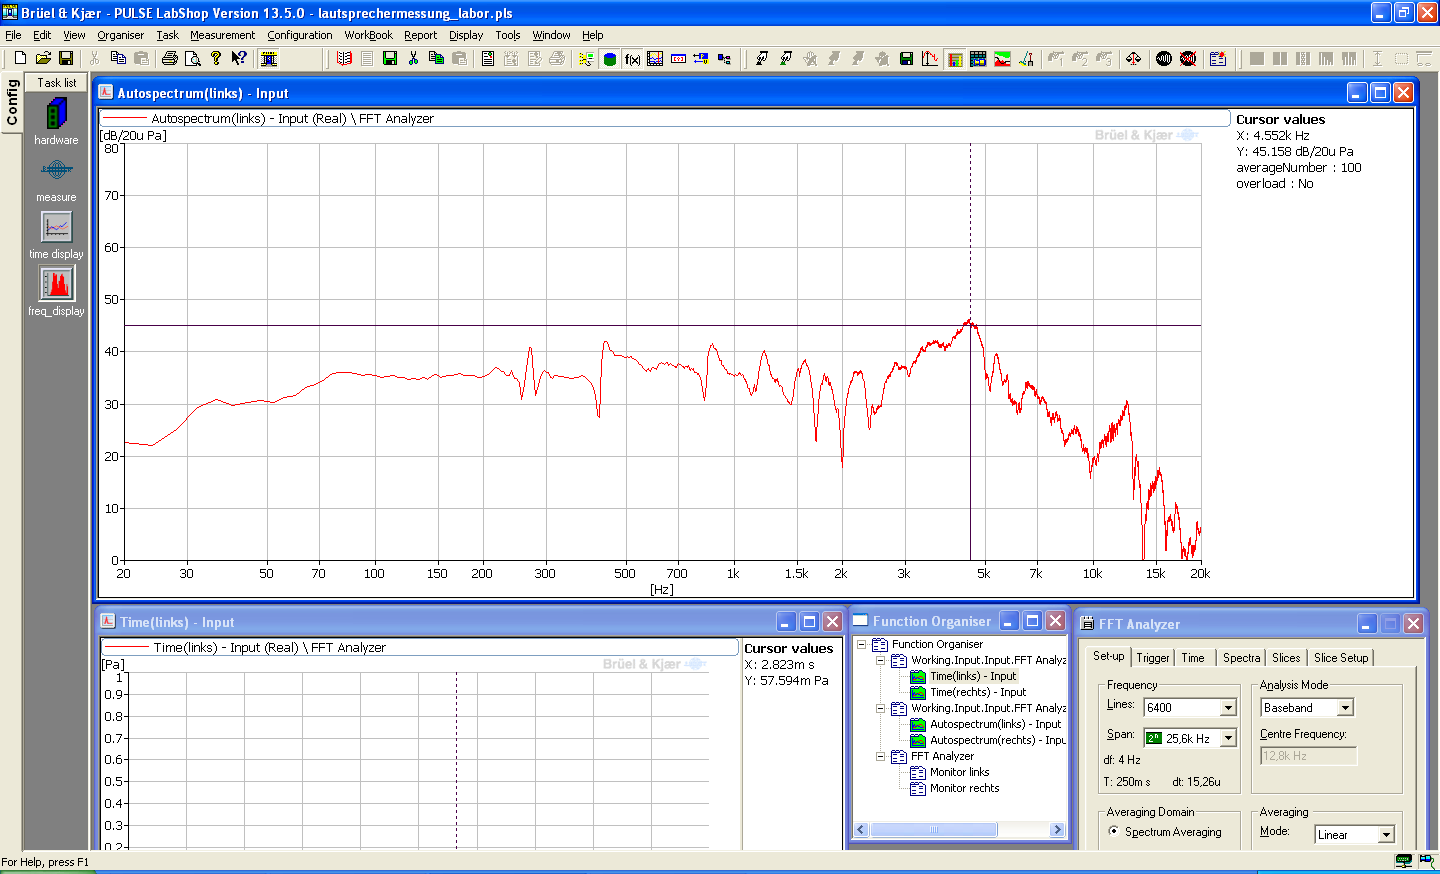
\includegraphics[width=0.75\textwidth]{img/LSMessung/TT/TT1mitSilikon.png}}\quad
	\subfloat{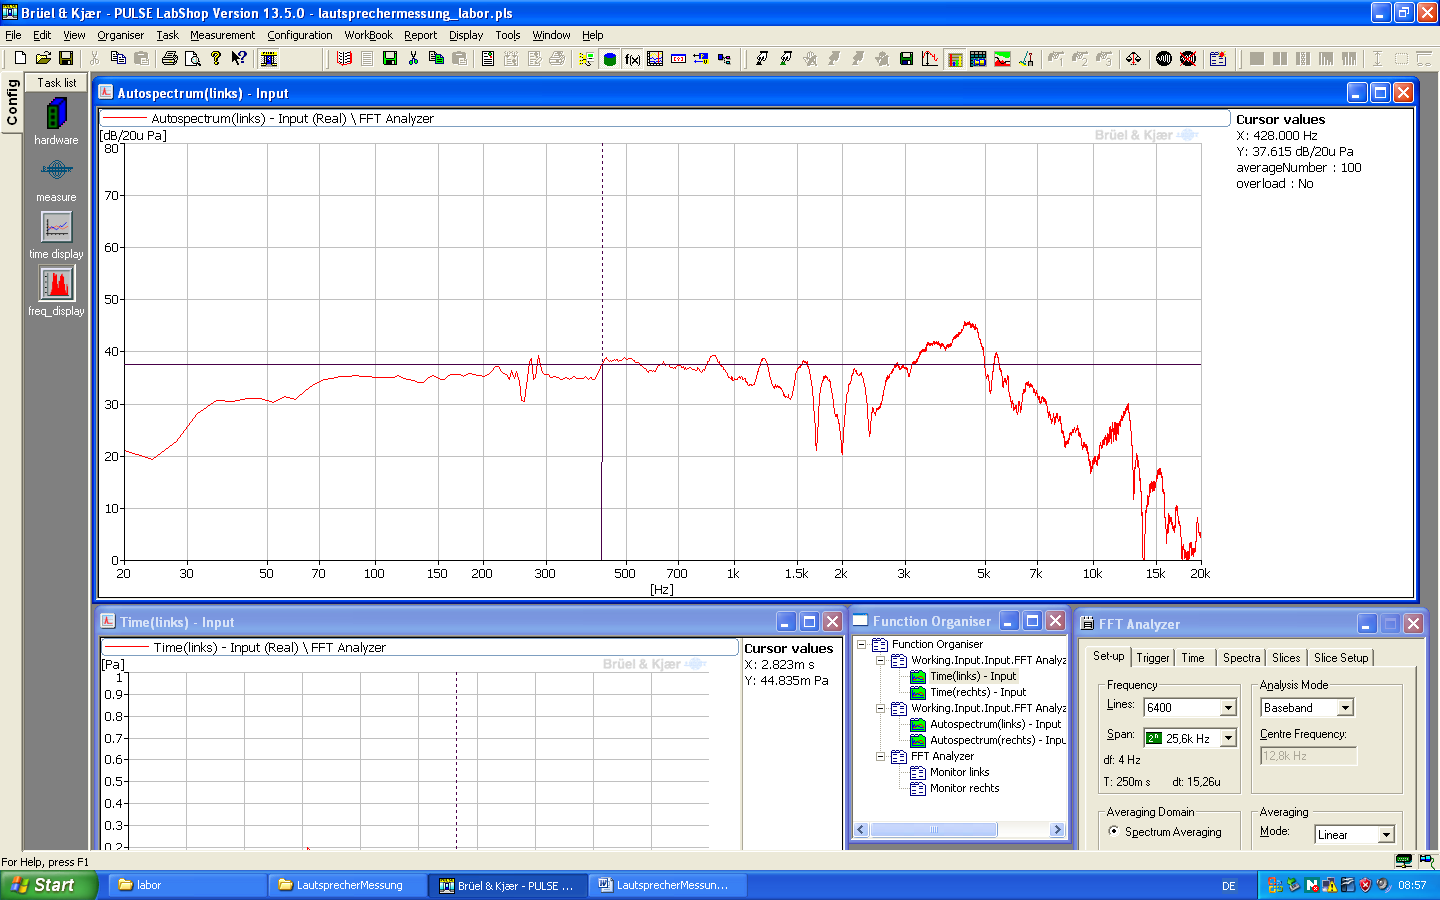
\includegraphics[width=0.75\textwidth]{img/LSMessung/TT/TT1mitSilikonUndWolle.png}}
	\caption{Tieftöner-Messung ohne Wolle\\ \enquote{TT1} (oben) und mit Wolle \enquote{TT1} (unten) Boxenvolumen: 13,72l}
	\label{fig:5.3.4.1}
\end{figure}
Es ist die Verringerung der Welligkeit im Teiftonbereich (<1kHz) sichtbar.
In dieser Situation sollte der Tieftöner im besten Fall bis 1kHz spielen.
Des weiteren sollte er besser mit Wolle versehen werden.













